\begin{figure}[!htb]
\begin{center}
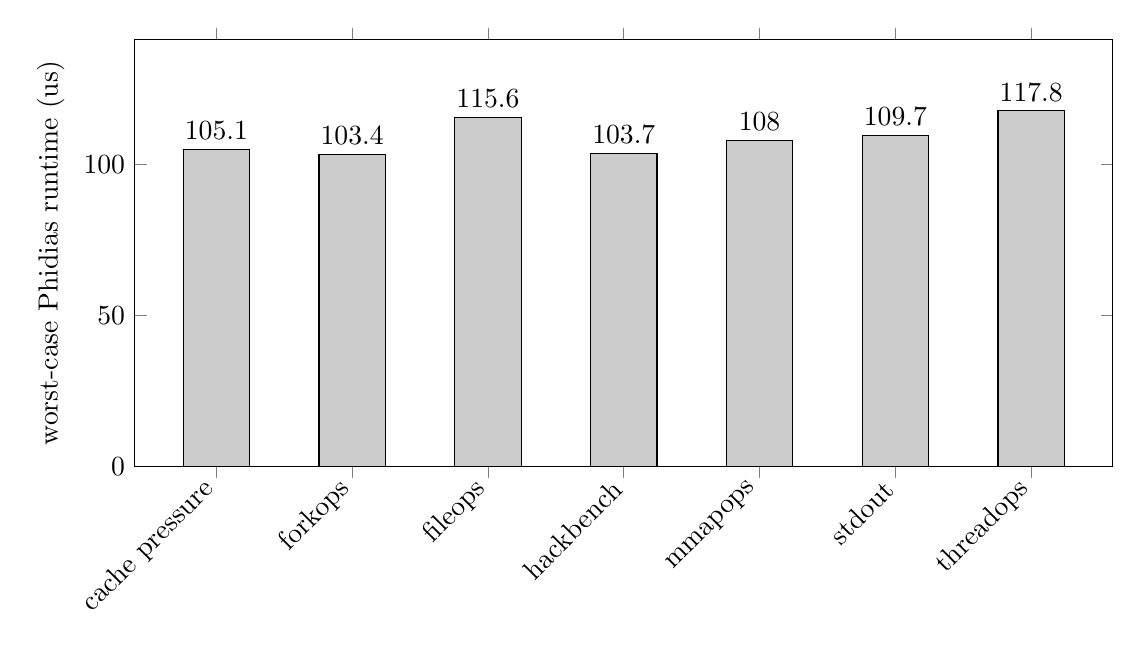
\begin{tikzpicture}

\begin{axis} [ ymin=0, ybar=2pt, height=7cm, width=14cm, enlarge y limits={upper,value=0.2}, 
		       legend style={at={(0.5,-0.3)}, anchor=north, legend columns=-1},
               ylabel={worst-case Phidias runtime (us)},
		       bar width=24pt,
  		       %%enlarge x limits={abs=0.8cm}, 		       
               symbolic x coords={no load, cache pressure,forkops, fileops, hackbench, mmapops, stdout, threadops, all benchmarks},
               xtick=data, nodes near coords, 
		       nodes near coords align={vertical},
		       %every node near coord/.append style={rotate=90, anchor=west},
               x tick label style={rotate=45,anchor=east}, ]    

			\addplot [fill=black!20] coordinates {				
				(cache pressure, 105.1)
				(forkops, 103.4)
				(fileops, 115.6)
				(hackbench, 103.7)
				(mmapops, 108)
				(stdout, 109.7)
				(threadops, 117.8)				
			    };
%\legend{}
\end{axis}

\end{tikzpicture}
\ifreport
\caption{Phidias runtime under different load conditions}
\fi
\end{center}
\label{plot-phidias-runtime}
\end{figure}
